\documentclass[10pt]{article}
\usepackage[letterpaper,textwidth=5.5in,top=0.85in,bottom=0.9in]{geometry}
\usepackage[T1]{fontenc}
\usepackage{newtxtext,newtxmath}
\usepackage{microtype}
\usepackage{graphicx}
\usepackage{caption}
\usepackage{booktabs,threeparttable,tabularx,array}
\usepackage{amsmath}
\usepackage{natbib}
\usepackage{tikz}
\usetikzlibrary{arrows.meta,positioning,shapes.geometric}
\usepackage{enumitem}
\usepackage{xurl}
\usepackage{float}
\usepackage[section]{placeins}
\usepackage[colorlinks=true,allcolors=blue!45!black]{hyperref}
\usepackage{cleveref}
\graphicspath{{figures/}}
\setlength{\parindent}{1em}
\setlength{\parskip}{0pt}
\setlength{\emergencystretch}{1.5em}
\captionsetup{font=small,labelfont=bf}
\makeatletter
\setlength{\@fptop}{0pt}
\makeatother

\newcommand{\pp}{\,\text{pp}}
\newcommand{\QwenWeak}{\texttt{qwen3.5:\allowbreak 9b}}
\newcommand{\Gemma}{\texttt{gemma4:\allowbreak 26b}}
\newcommand{\QwenStrong}{\texttt{qwen3.8:\allowbreak 27b}}
\newcommand{\Coder}{\texttt{qwen3-coder-next}}
\newcommand{\Llama}{\texttt{llama3.1:\allowbreak 8b}}
\newcommand{\Ornith}{\texttt{ornith1.5:\allowbreak 35b}}
\newcommand{\GLM}{\texttt{glm-5.3-flash}}
\newcommand{\GPT}{\texttt{gpt-5.6-sol}}
\newcommand{\SkillTraj}{\textsc{SkillTraj}}

\title{Cross-Model Analysis and Optimization of Agent Skills}
\author{Wang Qichen}
\date{}

\begin{document}
\maketitle

\begin{abstract}
Written skills tell coding agents how to inspect, edit, and validate repositories, but following a procedure need not produce a correct repair. This study introduces a fixed task pool and execution harness that records complete tool trajectories alongside external verifier outcomes. The main evaluation compared no skill (C0) with a fixed skill (C1) across 18 held-out tasks, eight model configurations, and 1,086 scheduled runs. C1 raised \GLM{} verifier pass from 74.1\% to 88.9\%, a task-paired gain of \(+14.8\)\pp{} with a 95\% bootstrap interval of \(\lbrack +3.7,+29.6\rbrack\)\pp{}. Effects for the other models were small or inconsistent. For \QwenWeak{}, C1 changed post-edit validation by \(-25.0\)\pp{}, while verifier pass changed by only \(+1.9\)\pp{}. A rewritten skill raised validation by 45.0\pp{} without changing pass. A follow-up experiment tested three procedural prompts against a length-matched generic control on 24 newly admitted development tasks (192 runs). Their task-paired pass differences were \(+6.3\), 0.0, and \(+4.2\)\pp{}. Every interval spanned zero, although the externalized procedure increased post-edit rereading by 31.3\pp{}. Across both studies, written instructions changed agent workflows without necessarily improving code, and outcome gains appeared only when instructions addressed remaining model-specific repair bottlenecks.
\end{abstract}

\section{Introduction}
Written skills give coding agents a procedure to follow when reading a repository, editing files, and checking their work. A skill succeeds at directing behavior when the agent follows those instructions. It succeeds at improving repair only when the resulting code meets the task requirements. These are separate questions. An agent may run more checks because it is working carefully, because an edit introduced a new error, or because repeated attempts have failed.

We compare a fixed skill (C1) with no skill (C0) across models, using the same task specifications, tools, verifiers, and fixed schedules. External verifiers determine whether each repair passes. Tool logs show how the agent reached that result. We also examine development runs and a qwen-only rewritten skill (v1) to understand which behaviors changed. Together, these measurements answer two questions: did the skill change what the agent did, and did its code pass more often?

The study makes three contributions:
\begin{enumerate}[leftmargin=1.4em,itemsep=1pt,topsep=2pt]
\item Introduce a frozen repository-repair task pool and execution harness that records complete tool trajectories alongside independently verified outcomes.

\item Provide a locked cross-model evaluation of written skills across 18 held-out tasks, eight model configurations, and 1,086 scheduled runs.

\item Identify a capability-dependent pattern: written skills offer little benefit at the performance floor or near a high-performing ceiling, while their greatest potential lies in models with sufficient task competence but remaining procedural weaknesses. Further showing that changes in agent behavior do not necessarily produce corresponding improvements in repair success.
\end{enumerate}

\section{Related Work}
Interactive language-model work has studied trajectories that alternate reasoning and actions. ReAct made such interleaving explicit and evaluated it across reasoning and interactive decision tasks \citep{yao2023react}. Our study takes the trajectory as an object of measurement, while asking a narrower question about fixed procedural instructions in repository repair.

Software-engineering agents are commonly evaluated through task completion against executable tests. SWE-bench uses real GitHub issues and repository-level changes with test-based evaluation \citep{jimenez2024swebench}; SWE-agent studies how an agent--computer interface changes software-engineering task performance and agent behavior \citep{yang2024sweagent}. Our task pool is synthetic and much smaller, but freezes each specification and verifier so the C0/C1 prompt contrast can be examined alongside detailed action traces.

Instruction-following evaluations provide complementary measures of compliance. IFEval emphasizes automatically checkable output constraints \citep{zhou2023ifeval}; AgentIF studies longer, constraint-rich instructions in agentic settings, including tool-related constraints \citep{qi2025agentif}. Compliance with a prescribed procedure and correctness of the resulting code are distinct outcomes. Our analysis measures both under a common repository-repair protocol rather than treating one as evidence for the other.

\section{Methods}
\subsection{Task pool and study design}
The project contains repository-repair tasks with a task statement, a buggy seed, fixtures, and an external verifier. Development data were divided into diagnosis and validation subsets; the held-out set comprised 12 \texttt{test\_in} tasks from Skills A/B and six \texttt{test\_out} tasks from Skill C. Admission checks required positive fixtures to pass and buggy or shortcut fixtures to fail the verifier.

The primary comparison paired C0 (no skill) with C1 (the frozen v0 skill). Eight model configurations were analyzed: \QwenWeak{}, \Gemma{}, \QwenStrong{}, \Coder{}, \Llama{}, \Ornith{}, \GLM{}, and \GPT{}. The seven non-GPT configurations used runner r2; \QwenWeak{} had five repetitions per task and all other C0/C1 configurations had three. Two qwen-only exploratory conditions were also run: a revised skill condition (v1) on the 12 \texttt{test\_in} tasks and a fixed call-32 reminder on all 18 tasks. The analyzed schedule contained 1,086 runs.

The schedule and outcome protocol were specified in a hash-locked, timestamped plan before the held-out evaluation. Conditions were interleaved using fixed per-model schedules. No task, verifier, fixture, or skill asset was changed during evaluation.

\subsection{Execution and outcomes}
Runner r2 recorded provider responses, parsed tool calls, command results, file edits, sampling metadata, terminal flags, and verifier outputs. It requested temperature 0.5, a seed when supported, up to 40 tool calls, a 65,536-token context budget, 120-second command timeouts, and a 1,200-second process-group timeout; metadata records requested and observed settings. Retry-exhausted provider errors were excluded from the primary pass-rate numerator and denominator. Hard timeouts and step-limit runs remained failures in the denominator. We report provider-error sensitivity with those runs counted as failures.

The primary outcome was the frozen Boolean \path{verifier.json.passed}, independent of the agent's final message. Terminal indicators such as \texttt{final\_empty}, \texttt{no\_edit}, and \texttt{timeout} were analyzed as non-exclusive process measures. A run with a final empty message could still pass the verifier.

\subsection{Statistical analysis}
The task was the sampling unit; repetitions estimated within-task variability. C0/C1 contrasts were task-paired and summarized by a fixed-seed, 10,000-draw paired bootstrap. Individual proportions use Wilson intervals. Wilson intervals describe single proportions and were not used as tests of between-condition differences. For process summaries, we report medians and interquartile ranges across task-level summaries, together with run-level occurrence rates where relevant.

Using observed within-task Bernoulli variance, approximate minimum detectable differences at two-sided \(\alpha=0.05\) and 80\% power ranged from 9.0 to 11.6\pp{} across the controlled three-repeat models. These estimates describe the sensitivity of this task pool under the stated assumptions; they are neither observed effects nor proof that smaller effects are absent.

\subsection{Fresh-task mechanism study}
We separately evaluated whether more explicit procedural prompts could change process behavior on 24 newly authored development tasks that passed the same admission requirements. This study used only \QwenWeak{} and compared four interleaved conditions: the v0 skill reference (C1), an externalized read--edit--validate--reread procedure, an abstract imitation of that sequence, and a 51-word generic control. Each task--condition cell had two repetitions, for 192 scheduled runs. The task pool, prompts, schedule, denominators, and analysis were locked before the first provider request. This development-only study does not revise the held-out comparison.

Each procedural condition was compared with the generic control after averaging repetitions within task--condition cells. Contrasts use a fixed-seed, 10,000-draw paired bootstrap over 24 tasks. The pre-specified efficacy rule required a positive pass-rate contrast with an interval excluding zero, observable activation, and no provider-error or timeout artifact. Mechanical process measures included validation after the last edit and rereading after an edit.

\subsection{Evaluation pipeline}
Tasks and verifiers were frozen before runs were interleaved. The harness recorded the execution trajectory, verified the final workspace, and paired outcomes by task for analysis (\cref{fig:pipeline}).

\begin{figure}[t]
\centering
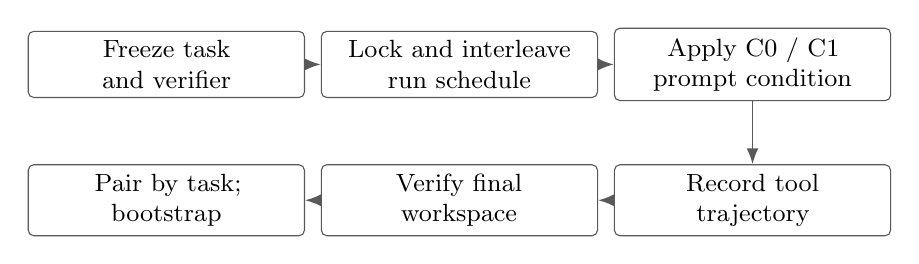
\begin{tikzpicture}[
  node distance=0.2cm,
  box/.style={draw=black!65,rounded corners=2pt,align=center,text width=0.27\textwidth,minimum height=0.78cm,font=\small},
  arrow/.style={-{Latex[length=2mm]},line width=0.6pt,draw=black!65}
]
\node[box] (freeze) {Freeze task\\and verifier};
\node[box,right=of freeze] (schedule) {Lock and interleave\\run schedule};
\node[box,right=of schedule] (prompt) {Apply C0 / C1\\prompt condition};
\node[box,below=0.8cm of prompt] (runner) {Record tool\\trajectory};
\node[box,left=of runner] (verify) {Verify final\\workspace};
\node[box,left=of verify] (analyze) {Pair by task;\\bootstrap};
\draw[arrow] (freeze) -- (schedule);
\draw[arrow] (schedule) -- (prompt);
\draw[arrow] (prompt) -- (runner);
\draw[arrow] (runner) -- (verify);
\draw[arrow] (verify) -- (analyze);
\end{tikzpicture}
\caption{Evaluation pipeline. The task pool contains 18 held-out tasks; the analyzed schedule contains 1,086 runs across eight model configurations and core/exploratory conditions. The inferential unit for C0/C1 comparisons is the task.}
\label{fig:pipeline}
\end{figure}

\section{Results}
\subsection{Cross-model verifier pass}
All 1,086 analyzed run directories contained metadata and a Boolean verifier result. The clearest positive result was \GLM{}: C0 passed 40/54 runs (74.1\%) and C1 passed 48/54 (88.9\%), yielding a task-paired difference of \(+14.8\)\pp{} with a 95\% bootstrap interval of \([+3.7,+29.6]\)\pp{} (\cref{tab:core,fig:main}). Its direction was positive on both held-out splits. The remaining controlled estimates were smaller or inconsistent. \Gemma{} increased by \(+5.6\)\pp{}; \QwenWeak{}, \QwenStrong{}, and \Coder{} each increased by \(+1.9\)\pp{}. \Ornith{} passed 45/52 usable C0 runs (86.5\%) and 44/52 C1 runs (84.6\%), a paired difference of \(-1.9\)\pp{} \([-16.7,9.3]\). Three Ornith records for \texttt{test\_out\_c02\_sessions} carried an alternate task-tree hash; each achieved \texttt{verifier.passed=true} and is counted as correct in the primary result. \Llama{} passed no held-out run, making its zero contrast a floor rather than evidence of equivalence. The GPT reference anchor had identical marginal pass counts under C0 and C1. Thus C1 produced a substantial gain for one model, little change for several models, and no rescue at the floor.

\begin{table}[t]
\centering
\scriptsize
\begin{threeparttable}
\caption{Verifier pass for the locked core conditions. The sampling unit for the contrast is the task; intervals are 95\% paired-bootstrap intervals over 18 tasks.}
\label{tab:core}
\begin{tabular}{@{}lrrr@{}}
\toprule
& \multicolumn{2}{c}{Verifier pass, runs} & Task-paired C1--C0 \\
\cmidrule(lr){2-3}\cmidrule(l){4-4}
Model & C0 & C1 & Difference (\pp) \\
\midrule
% PAPER_NUMBERS:CORE_BEGIN
\QwenWeak & 43/89 (48.3\%) & 45/89 (50.6\%) & \(+1.9\;[-6.9,10.6]\) \\
\Gemma & 33/54 (61.1\%) & 36/54 (66.7\%) & \(+5.6^\dagger\;[0.0,14.8]\) \\
\QwenStrong & 45/54 (83.3\%) & 46/54 (85.2\%) & \(+1.9\;[-3.7,7.4]\) \\
\Coder & 33/54 (61.1\%) & 34/54 (63.0\%) & \(+1.9\;[-7.4,13.0]\) \\
\Llama & 0/54 (0.0\%, floor) & 0/54 (0.0\%, floor) & \(0.0\;[0.0,0.0]\) (floor) \\
\Ornith & 45/52 (86.5\%) & 44/52 (84.6\%) & \(-1.9\;[-16.7,9.3]\) \\
\GLM & 40/54 (74.1\%) & 48/54 (88.9\%) & \(+14.8\;[+3.7,+29.6]\) \\
\GPT\tnote{a} & 44/54 (81.5\%) & 44/54 (81.5\%) & \(0.0\;[-5.6,5.6]\) \\
% PAPER_NUMBERS:CORE_END
\bottomrule
\end{tabular}
\begin{tablenotes}[flushleft]\footnotesize
\item[] \(\dagger\) The lower paired-bootstrap bound is exactly 0.0. Provider errors are excluded from primary denominators; the qwen denominators are 89 of 90 and the Ornith denominators are 52 of 54 scheduled runs per condition. All three alternate-hash Ornith records passed the frozen external verifier and are included as correct.
\end{tablenotes}
\end{threeparttable}
\end{table}

\begin{table}[t]
\centering
\small
\begin{threeparttable}
\caption{Verifier pass conditional on final-message status for held-out C0/C1 runs. The unit is a scheduled run; denominators include protocol provider-error records for this descriptive cross-tab (\(n=720\)).}
\label{tab:empty}
\begin{tabular}{@{}lrrrr@{}}
\toprule
Model & All runs & Final empty & Pass if empty & Pass if non-empty \\
\midrule
\QwenWeak & 180 & 105 (58.3\%) & 50/105 (47.6\%) & 39/75 (52.0\%) \\
\Gemma & 108 & 2 (1.9\%) & 1/2 (50.0\%) & 68/106 (64.2\%) \\
\QwenStrong & 108 & 0 (0.0\%) & 0/0 (NA) & 91/108 (84.3\%) \\
\Coder & 108 & 7 (6.5\%) & 3/7 (42.9\%) & 64/101 (63.4\%) \\
\Ornith & 108 & 6 (5.6\%) & 0/6 (0.0\%) & 89/102 (87.3\%) \\
\GLM & 108 & 0 (0.0\%) & 0/0 (NA) & 88/108 (81.5\%) \\
\bottomrule
\end{tabular}
\begin{tablenotes}[flushleft]\footnotesize
\item These are descriptive behavior rates; all scheduled records, including protocol provider-error records, are retained in these conditional denominators.
\end{tablenotes}
\end{threeparttable}
\end{table}



\begin{figure}[t]
\centering
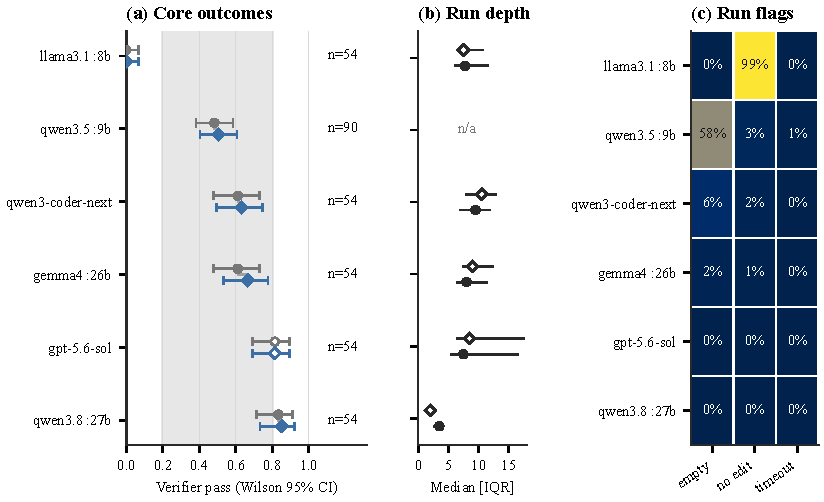
\includegraphics[width=\textwidth]{main_results.pdf}
\caption{Held-out task-pool results for eight model configurations. In panel (a), gray circles denote C0 and blue diamonds C1; pass rates use runs and Wilson 95\% intervals, while paired contrasts use tasks (18 task pairs per controlled model). Panel (b) shows medians and IQRs (filled circles: tool calls; open diamonds: assistant turns); panel (c) shows run-flag rates. Row-end \(n\) is the number of scheduled runs per condition (18 tasks by repetitions). Ornith is shown as recorded, with all verifier-passing records counted as correct; GPT is a sampling-uncontrolled reference anchor.}
\label{fig:main}
\end{figure}

\subsection{Process behavior and verified outcome}
For \QwenWeak{}, the task-paired rate of post-edit commands matching the strict validation rule was 25.0\pp{} lower under C1 than C0 (18 tasks; 95\% paired-bootstrap interval \([-38.9,-9.4]\)\pp{}). The baseline skill therefore reduced this checking behavior. In the exploratory \texttt{test\_in} comparison, v1 increased it by 45.0\pp{} over C1 (12 tasks; \([26.7,63.3]\)\pp{}). The pass-rate differences were much smaller: \(+1.9\)\pp{} for C1--C0 (\([-6.9,10.6]\)\pp{}) and \(0.0\)\pp{} for v1--C1 (\([-11.7,13.3]\)\pp{}). The rewritten skill led to more checking without a higher observed pass rate (\cref{fig:decoupling}).

\GLM{} showed a different coupling between process and outcome. C1 increased task-paired post-edit validation by 22.2\pp{} \([9.3,35.2]\) and increased the median trajectory from five to six tool calls. Over the same tasks, verifier pass increased by 14.8\pp{}. This is the only evaluated configuration in which the fixed skill produced a clearly positive overall pass-rate contrast together with a process change in the prescribed direction.

\begin{figure}[b]
\centering
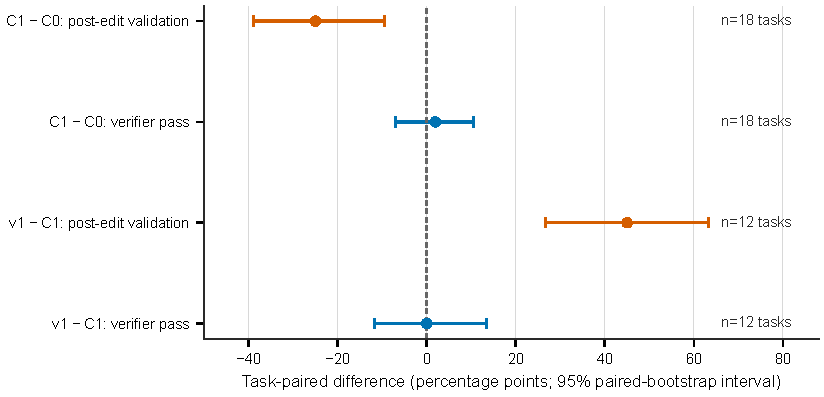
\includegraphics[width=0.62\textwidth]{decoupling.pdf}
\caption{Task-paired qwen contrasts for validation behavior and verifier pass. Intervals are 95\% paired-bootstrap intervals; the resampling unit is the task (\(n=18\) for C1--C0 and \(n=12\) for v1--C1). v1 is exploratory and limited to \texttt{test\_in}.}
\label{fig:decoupling}
\end{figure}

\subsection{Fresh-task process variants}
On the 24 fresh development tasks, the generic control passed 26/47 (55.3\%) usable runs. C1 passed 27/44 (61.4\%), the externalized procedure 25/47 (53.2\%), and imitation 26/45 (57.8\%). After pairing by task, their pass-rate differences from the generic control were \(+6.25\)\pp{} \([-8.33,+20.83]\), \(+0.00\)\pp{} \([-18.75,+18.75]\), and \(+4.17\)\pp{} \([-10.42,+20.83]\), respectively. Every interval included zero, so none met the pre-specified efficacy rule (\cref{fig:fresh}).

The process measures changed more clearly than the verified outcome. Relative to the generic control, the externalized condition increased task-paired post-edit rereading by 31.3\pp{} \([14.6,47.9]\) and validation after the last edit by 10.4\pp{} \([-4.2,25.0]\), while its pass difference was exactly 0.0\pp{}. Imitation increased rereading by 18.8\pp{} \([0.0,35.4]\) but changed validation by \(-2.1\)\pp{} \([-18.8,14.6]\). The locked activation parser also marked 46/47 generic-control runs as activated, so activation did not distinguish prompt conditions in this cohort. These results provide a fresh-task replication of process--outcome separation, not a new held-out efficacy claim.

\begin{figure}[t]
\centering
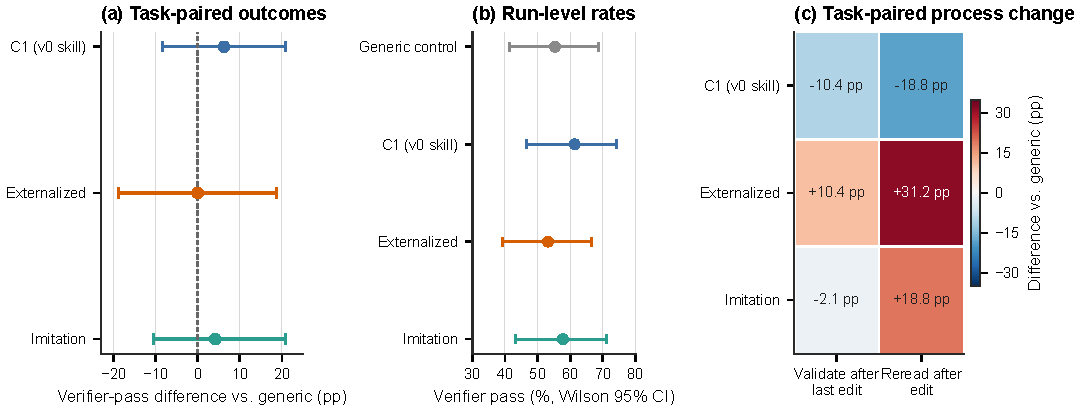
\includegraphics[width=\textwidth]{s8b_mechanism.pdf}
\caption{Fresh-task mechanism study on \QwenWeak{}. Panel (a) shows task-paired verifier-pass differences relative to the length-matched generic control with 95\% paired-bootstrap intervals (24 tasks; two repetitions per task--condition cell). Panel (b) shows run-level pass proportions with Wilson 95\% intervals; primary denominators exclude retry-exhausted provider errors. Panel (c) shows task-paired changes in validation and rereading relative to the generic control. The study contains 192 scheduled runs and is development-only.}
\label{fig:fresh}
\end{figure}

\subsection{Strong-versus-weak process summaries}
The strong comparison group contains \Gemma{}, \QwenStrong{}, and \Coder{}; the weak target is \QwenWeak{}. \Cref{tab:process} reports medians and IQRs across runs and run-level occurrence rates for binary behaviors. Under r2, each parsed tool result counts as one tool call, so step and call summaries coincide. The weak target's validation-intent occurrence fell from 64.0\% in C0 to 38.2\% in C1, whereas the strong cohort remained near 70\% in both conditions.
\begin{table}[t]
\centering
\scriptsize
\begin{threeparttable}
\caption{Strong and weak cohort process summaries under the core conditions. Values are median [IQR]; binary rates include run-level percentages in parentheses.}
\label{tab:process}
\setlength{\tabcolsep}{3pt}
\begin{tabular*}{\textwidth}{@{\extracolsep{\fill}}llrrrrrrr@{}}
\toprule
Cohort & Condition & \(n\) & Steps/calls & Turns & Intent & Success & Rewrites & Timeout \\
\midrule
% PAPER_NUMBERS:PROCESS_BEGIN
Strong & C0 & 162 & 8 [7,11] & 9 [7.2,12] & 100 [0,100]\% (68.5\%) & 100 [100,100]\% (93.8\%) & 0 [0,75] (25.3\%) & 0 [0,0]\% \\
Strong & C1 & 162 & 9 [7,12] & 9 [7,12] & 100 [0,100]\% (71.6\%) & 100 [100,100]\% (97.5\%) & 0 [0,0] (17.9\%) & 0 [0,0]\% \\
Weak & C0 & 89/90 & 8 [6,14] & 9 [7,15] & 100 [0,100]\% (64.0\%) & 100 [100,100]\% (86.5\%) & 0 [0,100] (40.4\%) & 0 [0,0]\% (1.1\%) \\
Weak & C1 & 89/90 & 7 [5,19] & 8 [6,20] & 0 [0,100]\% (38.2\%) & 100 [0,100]\% (65.2\%) & 0 [0,100] (31.5\%) & 0 [0,0]\% (1.1\%) \\
% PAPER_NUMBERS:PROCESS_END
\bottomrule
\end{tabular*}
\begin{tablenotes}[flushleft]\footnotesize
\item Values are median [IQR] across runs; parenthetical values are run-level rates. Intent is a command matching the frozen validation-intent rule; success is any successful command after the last edit. Under r2, one parsed tool result is one call, so steps and calls coincide. Strong includes three models; weak includes \QwenWeak{}. Weak usable runs exclude one retry-exhausted provider error per condition.
\end{tablenotes}
\end{threeparttable}
\end{table}

\subsection{Development behavior--outcome cross-tab}
The four-cell cross-tab uses only the development diagnosis subset, with mechanically defined behaviors and verifier outcomes. Reading before editing occurred in every cell. In both model cohorts, post-edit validation and rereading were at least as common among failures as among passes, while avoiding repeated full-file writes changed little across outcomes (\cref{tab:crosstab,fig:behavior}). This does not imply that validation harms repair: difficult runs may require more checking, and the cells are observational. It does show that these individual checklist behaviors did not distinguish successful from failed runs in this sample. The weak pass and weak fail cells contain only 10 and 8 runs.

\begin{table}[t]
\centering
\small
\begin{threeparttable}
\caption{Mechanical behavior rates in the development diagnosis subset. Values are count/usable runs (percentage); cells are observational strata.}
\label{tab:crosstab}
\begin{tabular}{@{}lrrrr@{}}
\toprule
Behavior & Strong pass & Strong fail & Weak pass & Weak fail \\
\midrule
% PAPER_NUMBERS:CROSSTAB_BEGIN
Read before edit & 47/47 (100.0\%) & 6/6 (100.0\%) & 10/10 (100.0\%) & 8/8 (100.0\%) \\
Validate after edit & 33/47 (70.2\%) & 6/6 (100.0\%) & 3/10 (30.0\%) & 5/8 (62.5\%) \\
Avoid repeated full-file write & 36/47 (76.6\%) & 5/6 (83.3\%) & 8/10 (80.0\%) & 6/8 (75.0\%) \\
Reread after edit & 12/47 (25.5\%) & 3/6 (50.0\%) & 2/10 (20.0\%) & 4/8 (50.0\%) \\
% PAPER_NUMBERS:CROSSTAB_END
\bottomrule
\end{tabular}
\begin{tablenotes}[flushleft]\footnotesize
\item Strong comprises three fixed models; weak is \QwenWeak{}. One retry-exhausted run is excluded. No interval is reported for these descriptive cells.
\end{tablenotes}
\end{threeparttable}
\end{table}

\begin{figure}[t]
\centering
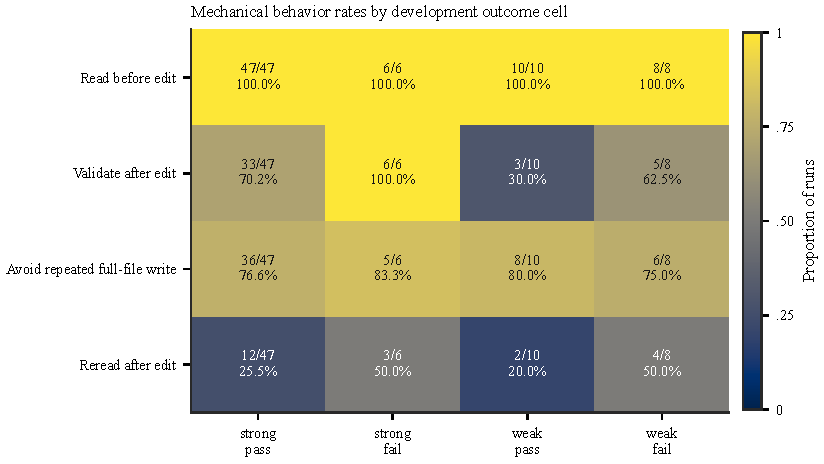
\includegraphics[width=\textwidth]{behavior_outcome.pdf}
\caption{Development diagnosis behavior--outcome cross-tab. Cell sample sizes are 47, 6, 10, and 8 runs (strong-pass, strong-fail, weak-pass, weak-fail); labels show count and percentage. No inferential interval is shown.}
\label{fig:behavior}
\end{figure}

\FloatBarrier
\subsection{Mechanical failure classification}
The weak-target, original stronger-model, Ornith, and GLM failure cohorts contain 98, 97, 15, and 20 verifier-failing usable runs, respectively. A run can appear in several flag columns; these counts describe failure contexts, not mutually exclusive causes.

\begin{table}[!t]
\centering
\small
\begin{threeparttable}
\caption{Non-exclusive mechanical failure flags among verifier-failing runs.}
\label{tab:failure}
\begin{tabular}{@{}lrrrrrr@{}}
\toprule
Cohort & \(n\) & No edit & Empty & Timeout & Compile & Step limit \\
\midrule
Weak development diagnosis & 8 & 0 & 3 & 0 & 0 & 0 \\
Weak target, held-out C0 & 46 & 4 & 27 & 1 & 1 & 5 \\
Weak target, held-out C1 & 44 & 2 & 27 & 1 & 1 & 8 \\
Weak target, combined & 98 & 6 & 57 & 2 & 2 & 13 \\
Three stronger models, held-out & 97 & 3 & 5 & 0 & 0 & 5 \\
\Ornith{}, held-out & 15 & 1 & 2 & 1 & 0 & 1 \\
\GLM{}, held-out & 20 & 0 & 0 & 0 & 0 & 0 \\
\bottomrule
\end{tabular}
\begin{tablenotes}[flushleft]\footnotesize
\item A run may contribute to more than one flag. The stronger group combines \Gemma{}, \QwenStrong{}, and \Coder{}; \Ornith{} and \GLM{} are shown separately because they were added after that pooled cohort was specified. Named failed verifier checks are summarized separately in the released mechanical taxonomy.
\end{tablenotes}
\end{threeparttable}
\end{table}

Among 98 verifier-failing weak-target runs from development diagnosis and held-out C0/C1, 57 ended with an empty final message, 13 reached the step limit, two timed out, and two produced a compile error. Among 97 held-out failures from the three stronger configurations, five reached the step limit and five ended with an empty final message. These overlapping flags identify where failures occurred in the execution record; they do not by themselves identify the error in the proposed code. Named verifier-check failures and verifier-exception categories are documented in the released mechanical taxonomy. The earlier judge packets cover none of these 98 weak-target failures, so \cref{fig:failures} uses mechanical indicators only.

Judge labels are used as conclusion evidence only for file corruption, tool misuse, and missed constraints; validation and looping claims rely on mechanical indicators.

\begin{figure}[t]
\centering
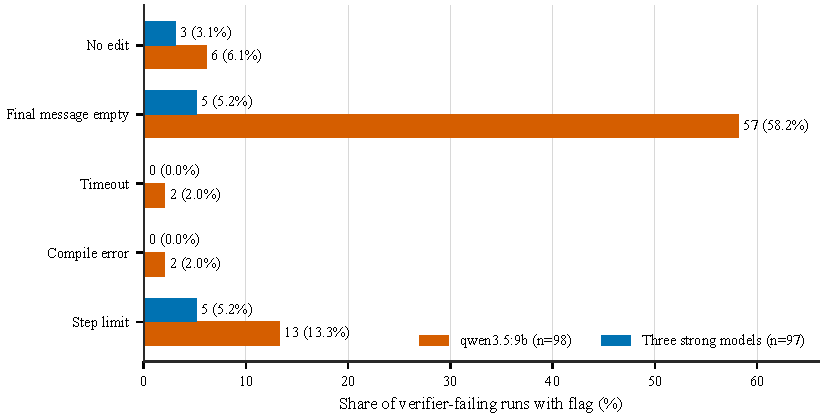
\includegraphics[width=\textwidth]{failure_flags.pdf}
\caption{Mechanical terminal flags among verifier-failing runs. Bars show the percentage of runs in each cohort carrying a flag; flags are non-exclusive and counts are printed beside each bar. Denominators are 98 weak-target failures and 97 failures from three stronger models; no interval is shown.}
\label{fig:failures}
\end{figure}
\FloatBarrier

\section{Discussion}

The results show that the usefulness of a written skill depends on the model's operating range. At the performance floor, \Llama{} passed no held-out run under either condition, so procedural instructions did not compensate for failed task execution. At the other end, \QwenStrong{}, \Ornith{}, and the GPT reference already exceeded 80\% under C0 and received no positive overall gain from C1. The strongest benefit appeared for \GLM{}, whose 74.1\% C0 baseline left room for improvement: C1 raised pass to 88.9\%, a task-paired increase of 14.8\pp{}. \Gemma{} showed a smaller \(+5.6\)\pp{} estimate, while the weak target and coder changed by only \(+1.9\)\pp{}. The pattern is not a monotonic function of model size; it depends on whether the model can execute the procedure and whether the prescribed actions address its remaining errors.

Changes in agent behavior did not reliably translate into better repairs. For \QwenWeak{}, C1 reduced post-edit validation by 25.0\pp{} while increasing verifier pass by only \(1.9\)\pp{}. The rewritten skill reversed the behavioral effect, increasing validation by 45.0\pp{} relative to C1, but produced no change in verifier pass. The development trajectories showed the same separation. Reading before editing was universal, while validation and rereading occurred at least as often in failed runs as in successful runs. Completing more prescribed steps therefore did not distinguish correct repairs from incorrect ones.

This separation matters because process compliance and task competence measure different properties. A model may follow a validation instruction yet test the wrong behavior, misinterpret a failure, or preserve an incorrect implementation. Conversely, a capable model may solve a task without explicitly displaying every requested step. The GLM result shows the positive case: the skill increased focused post-edit validation and repair success on the same task pool. The qwen v1 result shows the counterexample: a larger behavioral change did not improve correctness. A written skill helps only when its procedural guidance changes a decision that currently limits the repair.

The fresh-task mechanism study sharpens this interpretation. An externalized procedure increased post-edit rereading by 31.3\pp{}, yet its paired pass difference from a length-matched generic prompt was exactly 0.0\pp{}. Imitation also increased rereading without a pass interval excluding zero. These prompts changed observable checking behavior, but they did not establish a verified repair gain. The near-universal activation assigned to the generic control further shows that broad action detectors cannot substitute for condition-specific evidence of instruction use.

Skill evaluation should therefore measure three components together: whether the skill was delivered and followed, how it changed the execution trajectory, and whether the resulting artifact passed an independent verifier. Comparing only final pass rates hides whether the skill affected behavior, whereas comparing only trajectories can mistake procedural compliance for improved capability. Future skill design should target model-specific failure modes and should be evaluated within the capability range where the model can execute the procedure but has not already internalized it.

A useful skill evaluation must answer both questions. Tool logs reveal whether an agent followed the instruction; an external verifier determines whether its repair worked. Reporting only behavior can reward an agent for completing steps that do not fix the bug. Reporting only pass rate hides whether the skill changed the process at all. Our evaluation records both, so a change in checking behavior can be distinguished from a change in repair success.

Success is read directly from \path{verifier.json.passed}, with empty messages, step limits, and timeouts recorded separately. Earlier labels undercounted passing runs with empty final messages; the full correction history is documented in the \href{https://github.com/77chenchen/cross-model-analysis-and-optimization-of-agent-skills/blob/main/docs/verifier_pass_erratum_20261010.md}{repository audit}. The nine transport failures that exhausted their retries are excluded from the main denominator and counted as failures in the sensitivity analysis.

\section{Conclusion}

This study establishes a model-dependent operating range for written agent skills. The fixed skill materially improved \GLM{} on this task pool, raising verifier pass from 74.1\% to 88.9\% while increasing focused post-edit validation. The same skill did not rescue the floor model and did not improve the already high-baseline Ornith configuration. A skill is therefore most useful when the model already has enough task competence to execute the procedure but still has a procedural weakness that the instruction directly addresses.

The experiments also show that changing an agent's workflow is not automatically equivalent to improving its repairs. The rewritten skill substantially increased post-edit validation for \QwenWeak{}, yet its verifier pass rate remained unchanged. In contrast, GLM combined a smaller behavioral shift with a clear pass-rate gain. A successful skill must therefore do more than produce a better-looking trajectory: it must change the decisions that determine whether the final artifact is correct. Written skills should be designed for a specific model and failure regime, then evaluated using both complete execution trajectories and independent outcome verification.

The fresh-task study reaches the same measurement conclusion under a new task pool and a length-matched control. Explicitly externalizing the read--edit--validate--reread sequence increased rereading by 31.3\pp{} but changed task-paired verifier pass by 0.0\pp{}. This isolates the central distinction: a prompt can successfully redirect the workflow without improving the repair.

The conclusion from these experiments is direct: following the requested procedure is not enough to establish that a skill improves repair. A skill can change the steps an agent takes while leaving its success rate unchanged. Skill evaluation must therefore report what the agent did and whether the resulting code passed independent checks. A procedure should be credited with improving repair when the repairs improve, rather than when its checklist is completed more often.



\clearpage
\section*{Code and Data Availability}
Analysis code, released study data, locked configurations, and the scripts used to reproduce the tables and figures are available at \url{https://github.com/77chenchen/cross-model-analysis-and-optimization-of-agent-skills}. Source code is licensed under the MIT License; released data and documentation are licensed under CC BY 4.0. Raw provider responses containing private reasoning traces are not included in the public package.

\bibliographystyle{plainnat}
\bibliography{references}

\end{document}
